\chapter{Robots Móviles y Agentes Inteligentes}


\section{Máquina de Estado}

\begin{itemize}
	\item[\textbullet] Entradas
	\item[\textbullet] Máquinas
	\item[\textbullet] Salidas
\end{itemize}

\section{Máquina de Estado Aumentada}

Una entrada (o salida) de una máquina puede ser sustituida por la salida de otra máquina de estados. Esa bloquea la entrada (o salida) ordinaria y pone su salida.

\begin{figure}[h!]
	\centering
	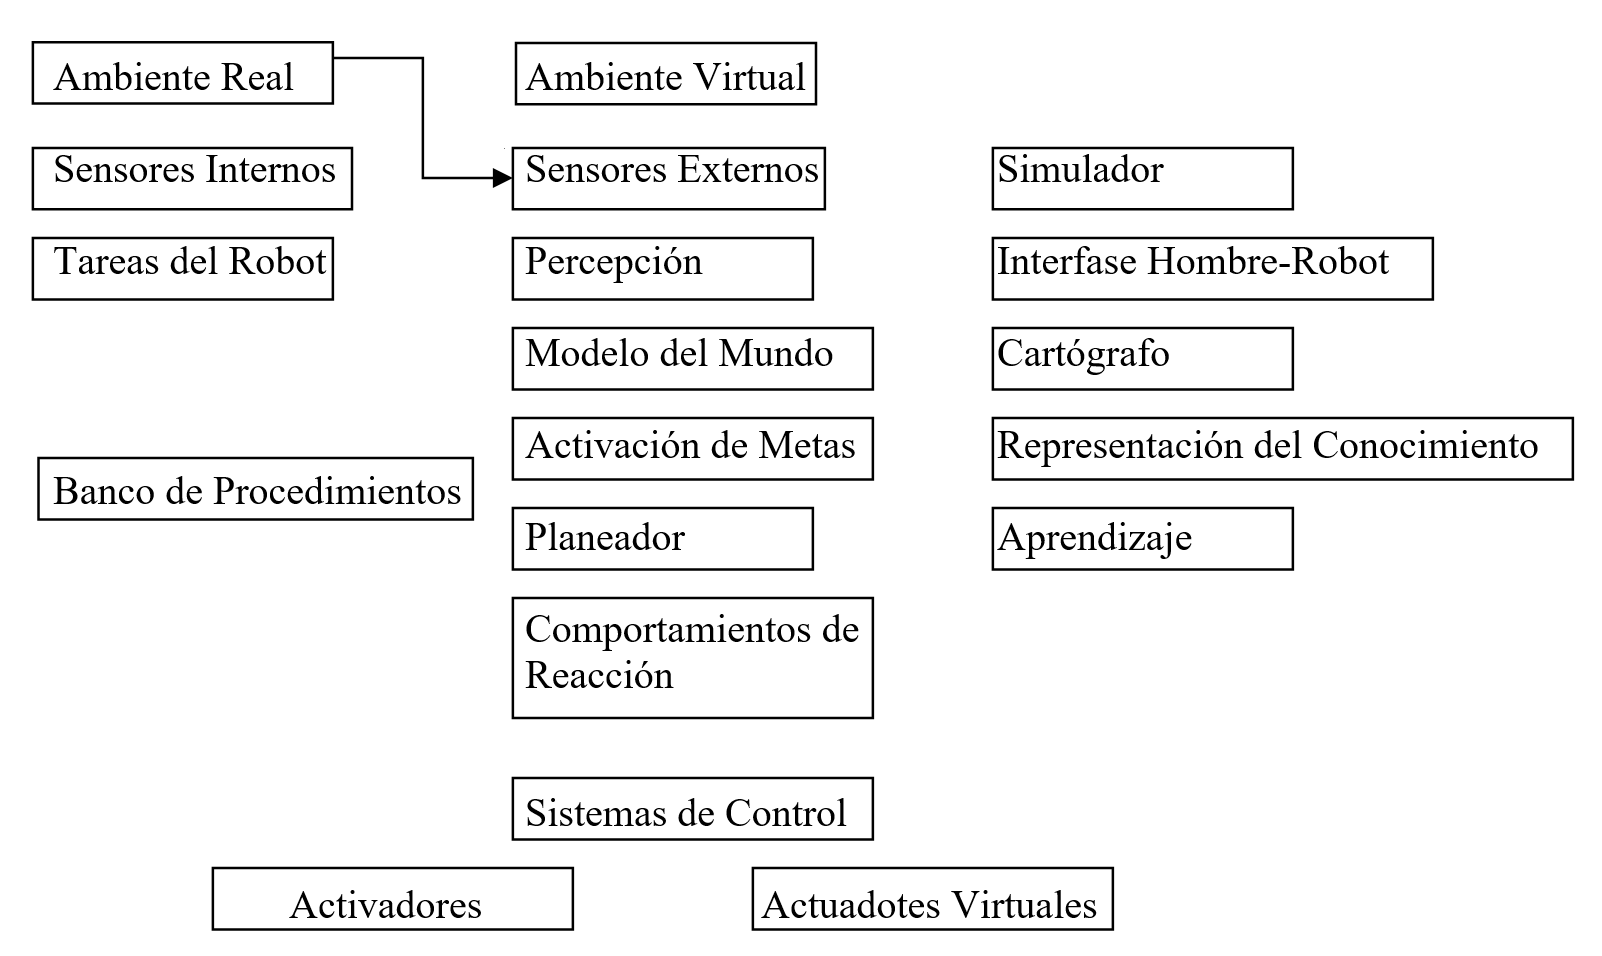
\includegraphics[width=0.5\textwidth]{images/img49.png}
	\label{figura49}
\end{figure}

\section{Arquitecturas Reactivas (o por Comportamientos)}

Diagramas de Stimulus Response (SR)

\begin{figure}[h!]
	\centering
	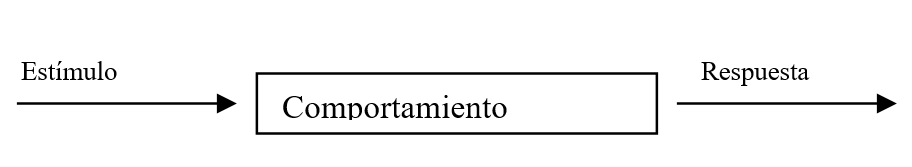
\includegraphics[width=0.5\textwidth]{images/img50.png}
	\label{figura50}
\end{figure}

La idea es que la respuesta sea instantánea.
En los comportamientos puros, la respuesta únicamente depende del estímulo.

\subsection{Organización de los comportamientos:} 

%imagen

Algunos comportamientos bloquean la salida de otros. Solamente la salida de uno es el que se usa, todos se activan. El diagrama anterior decide la prioridad.

La salida generalmente es un vector que, por ejemplo, indica la magnitud y dirección del movimiento del robot.

%imagen

El árbitro decide cuál es la respuesta.

%imagen

El sumador hace un promedio ponderado por ganancias.

$$
\sum_{i=1}^{N} \, g_i \, R_i
$$

La ganancia depende del diseñador y va a hacer que el robot se comporte de diferente forma (robot “audaz” contra robot “conservador”).

Un diagrama del espacio se puede hacer con campos vectoriales (diagramas de flechitas tipo sistemas dinámicos), por ejemplo uno que sea de las fuerzas de atracción y otro de repulsión y sumarlos.

Puedo tener una complejidad grande combinando comportamientos, pues pueden controlar diferentes cosas.


\section{Máquinas de Estado}
\subsection{Algoritmo para el Comportamiento de Evadir Obstáculos}

Un robot circula con:

\begin{itemize}
	\item[\textbullet] Dos motores, uno a cada lado.
	\item[\textbullet] Dos sensores adelante, para detectar obstáculos (por ejemplo, infrarrojos, ultrasonido, etc.)
\end{itemize}

%imagen

Obviamente:
\begin{itemize}
	\item[\textbullet] Si los sensores no detectan el obstáculo, seguir 		avanzando.
	\item[\textbullet] Si el sensor derecho lo detecta y el otro no, hacerlo tantito para atrás y girar hacia la izquierda para seguir avanzando
	\item[\textbullet]Si el sensor izquierdo lo detecta y el otro no, hacerlo tantito para atrás y girar hacia la derecha para seguir avanzando
	\item[\textbullet]Si los dos detectan, hacerlo para atrás y giro 90°.
\end{itemize}

%imagen

\textit{Notación de diagrama de flujo}

%imagen

Si se quisiera programar esto con una subrutina, hace todo.  En la teoría de comportamientos necesito una respuesta inmediata y necesito que cuando vuelva a entrar se guarde el estado.

\section{AFSM (Augmented Finite State Machine)}

La máquina de estados aplicada a robots representa el comportamiento.
Una máquina tradicional de estados tiene entradas y salidas.
Rodney Brooks (MIT) inventó la máquina de estados finitos aumentada.

Básicamente el concepto es que alguna de las entradas es inhibida por otra máquina de estados (su salida se convierte la entrada) y en las salidas están los supresores, que bloquean la salida de la máquina y colocan un valor. Por último hay una entrada de “reset” que hace que se coloque en un estado en específico.

Con AFSM podemos tener diferentes capas y hacer una respuesta \textbf{jerárquica}.

%imagen

\section{Campos Potenciales}

Se modela el robot como una canica. Los obstáculos ahora son montañas que ejercen fuerzas de repulsión. El destino es un hoyo.
El robot se mueve a través de un campo potencial por la pendiente más pronunciada hasta que lo lleva al destino.

%imagen
$$
y=y_0 + (x-x_0)^2
$$

El mínimo se encuentra diferenciando.

$$
x^* = x_0
$$

Supongamos que no se conoce la ecuación; entonces se utiliza un método iterativo.
Empiezo con un punto $x_{n-1}$ cualquiera y dependiendo del valor de la pendiente me muevo hacia la izquierda o la derecha.

Es una relación de recurrencia:

%formula 

\textbf{Por ejemplo:} \\
Si consideramos $\delta = \dfrac{1}{2}$ se tiene $x_n = x_{n-1} \, \dfrac{-1}{2}(2(x_{n_1}-x_0)) = x_0$.


Esto da pie a considerar la situación general.

\textbf {Se utiliza Steepest Descent.} 

Posición del robot en n: $q_n = \left[x_n,y_n\right]^T$
$$
q_n=q_{n-1}-\delta f (q_{n-1}) $$

donde $f(z)= \dfrac{F(z)}{\|F(z)\|} = U(z)$ y $U(z)$  es el campo potencial del medio ambiente en donde navega el robot $U(z)= U_{atr}(z) + U_{rep}(z)$ (dos componentes, uno atractor y un repulsor).

Al final se tienen fuerzas de atracción más fuerzas de repulsión.

Se define:

$U_{atr} = \dfrac{1}{2} \, \varepsilon_1 \,  \|q-q_{dest}\|^2 $(campo de tipo parabólico) donde $q_{dest}$  es la posición del destino. 
Se ve claro que es parabólico:

$$
U_{atr}=\frac{1}{2} \, \varepsilon_1(x-x_{dest})^2 + (y-y_{dest})^2
$$
La fuerza de atracción en q es:

$$
U_{atr}= \varepsilon_1 
$$


La fuerza de atracción se va a convertir en aceleración. Para fuerzas muy grandes se transforma en aceleraciones muy grandes. 
Esto no se quiere, por lo que se tiene un umbral. Esta fórmula solamente aplica para $\|q-q_{dest}\| < d_1$.

¿Qué pasa en $\|q-q_{dest}\|>d_1$?

$$
U_{atr}=E_2\|q-q_{dest}\|
$$

Esto es un campo cónico:

$$
U_{atr}=E_2\sqrt{(x-x_{dest}^2 + (y-y_{dest})^2)}
$$

$$
U_{atr}=E_2
$$

Campos Repulsivos
¿Cómo representar el obstáculo? Se podría considerar un solo vector en el centroide, una serie de puntos que ejercen repulsión, etc. Depende del diseñador.

$$
U_{rep}(q)=\frac{1}{2} \eta
$$

Esto aplica cuando $\|q-q{obs} \|$. En caso contrario, se toma como 0. Esto es para que no lo tomes en cuenta si está demasiado lejos.

$$
U_{rep}(q)=F_{rep}(q)
$$

En general,

$$
F(q)=F_{atr}(q)+\sum_{i=1}^{n}\, F_{rep}(q)
f(q)=\frac{F(q)}{\|F(q)\|}
q_{i+1}=q_i - \delta_i f(q_i)
$$

%imagen
\begin{ejemplo}
	Robot:(1,1) \\
	Obstáculo: hexágono centrado en (2,2) \\
	Objetivo:(5,4) \\
	$q_0=(1,1)$\\
	Se va a tomar $d_0=	5, \varepsilon_1=1, \eta=2,\delta_0=1$ y se va a utilizar la parabólica
\end{ejemplo}

Se tiene: 
$$
F_{atr}(q_0) = \varepsilon_1 (q_0-q_{dest}) = (-4,-3)
F_{rep}(q_0) = -(0\ldotp3585,0\ldotp3585)
$$

La fuerza total es: 

$$
F(q_0) = (-3\ldotp64,-2\ldotp64) \hspace{0.5cm} f(q_0)=(-0\ldotp8091,-0\ldotp 5868)
$$
Finalmente:

$$
q_1=q_0-\delta_0 f(q_0)
	=(1,1)+(0\ldotp8091.0\ldotp5868)
	=(1\ldotp8091,1\ldotp5868)
$$
Obsérvese que no hemos considerado la \textbf{orientación inicial del robot}.


¿Cómo encontrar las constantes? Empíricamente

Nota: Si no conocemos obstáculos no podemos calcular las fuerzas de repulsión. En estos casos, se tiene que usar la información de los sensores para identificar al obstáculo y, con base en eso, calcular estas fuerzas.

\textbf{Cálculo de los vectores de repulsión usando la posición de los obstáculos fijos}

Los obstáculos conocidos se representarán por polígonos que tienen nodos ordenados en el sentido de las manecillas del reloj.

El espacio se divide en celdas y en cada celda se calcula la fuerza total de repulsión.

%imagen

Etc.

¿Cómo encontrar la fuerza de repulsión en cada celda?

%imagen

El punto $x_r,y_r$ es el centro de la celda en donde se está (se asume que el robot está en el centro de la celda).

El punto $(x_f,y_f)$ es  un punto arbitrario (se quiere calcular para la mayor cantidad de direcciones posibles. No es en línea sino que se hace offline).

$$
L_1:\colon y=m_1x+b_1
L_R:y=m_Rx+b_R
$$

Nótese que 

$$
x_f=d\cos\phi+x_r
y_f=d\sin\phi+y_r
$$

Donde el ángulo es entre el eje x y la línea $L_R$.

Obs: se puede encontrar

$$
m=\frac{y_1-y_0}{x_1-x_0} \hspace{0.5cm} b=\frac{x_1y_0-y_1x_0}{x_1-x_0}
$$

Los puntos de intersección son

$$
x_{int}=\frac{b_r-b_1}{m_1-m_r} \hspace{0.5cm} y_{int}=m_r x_{int} + b_r
$$

Obsérvese que se tiene que cumplir que
\section{Cómo calcular el campo potencial para el caso de objetos desconocidos}

Lo anterior se hace offline y se alimenta al robot. Si hay objetos desconocidos:

%imagen

El ángulo theta es el eje principal del robot. El ángulo alpha es el ángulo entre el eje y el sensor.


$
x_{obs}=d\cos(\phi+\alpha) \\ y_{obs}=d\sin(\phi+\alpha) \\ \\
q-q_{obs}=(0,0)-(x_{obs},y_{obs})=(-x_{obs},-y{obs})
$

(puesto que se cambia el eje de coordenadas).

¿Qué se quiere?
De $(x_{i-1},y_{i-1},\phi_{i-|})$ (donde está el robot) necesito llegar a $(x_i,y_i,\phi_i)$.

Obsérvese que:

 $
 x_i=x_{i-1}+x_i \cos(\phi_i)
 y_i=y_{i-1}+x_i \sin(\phi_i)
 $
 
donde:

$
\phi=\phi_{i-1}+\phi_i \\
\phi=\arctan\ (\frac{y_i -y_{i-1}}{x_i -x_{i-1}})
$


Esto se conoce como \textbf{computación directa}.

Otra opción es:

$
\phi=\arctan\ (\frac{y_i -y_{i-1}}{x_i -x_{i-1}})
$


y obviamente también se tiene que 

Esto se llama computación inversa y es la que nos interesa.




Ejemplo


Esto se conoce como computación directa.

Otra opción es:



y obviamente también se tiene que 

Esto se llama computación inversa y es la que nos interesa.


